\documentclass[12pt,hyperref={unicode}]{beamer}
\usetheme{CambridgeUS}
\usepackage[utf8]{inputenc}
\usepackage{amsmath}
\usepackage{amsfonts}
\usepackage{amssymb}
\usepackage{lmodern}
\setbeamercolor{section number projected}{bg=brown,fg=black}
\setbeamercolor{subsection projected}{fg=brown}

\author{Burcu Alakuş}
\title{Steganography and Its Applications}
%\setbeamercovered{transparent} 
%\setbeamertemplate{navigation symbols}{} 
%\logo{} 
\institute{Atılım University} 
\subject{MATH 411 - Seminar Studies} 
\begin{document}

\begin{frame}
\titlepage
\end{frame}

\begin{frame}{Outline}
\centering
\tableofcontents
\centering
\end{frame}

%%%%%%%%%%%%%%%%%%%%%%%%%%%%%%%%%%%%%%%%%%%
\section{Introduction}
\begin{frame}
\begin{figure}
    \centering
    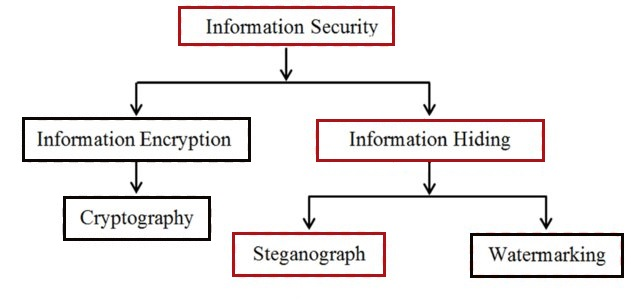
\includegraphics{Fig-7-Classification-of-the-security-system-41-Watermarking-Techniques-Digital_W640.jpg}
    \caption{Caption}
    \label{fig:my_label}
\end{figure}
\begin{center}
Cryptography: private and confidential\\ Steganography: provides the secrecy of communication.
\end{center}
\end{frame}

%---------------------------------------

%\begin{frame}

%Cryptography: a result of mathematical calculations that the reader and the analyser cannot understand.\\ Third parties cannot make sense of the message at first.\\ %Requires a significant time and effort.\\ 
%The main idea: to make it as hard as possible for third parties to resolve the message sent.
%\end{frame}

%---------------------------------------

\begin{frame}
\textbf{Steganography:} not to take the precaution, but to send it by concealing the message completely.\\ 
%Many methods and tools used to do that.\\
The message is sent to a carrier hiding in a way that does not attract attention.\\
%In cryptography, it is visible and attracts the attention and third parties' interest.\\
\begin{figure}[h]
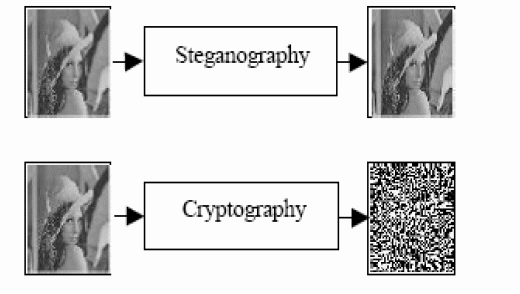
\includegraphics[width=7cm, height=4cm]{stego & kripto.png}
\caption{Steganography vs. Cryptography}
\end{figure}
\end{frame}

%---------------------------------------

%\begin{frame}
%Steganography techniques have been used in many fields throughout history.\\
%Steganography techniques can be used and was used in pre-war preparations, wars, political and diplomatic talks, intelligence activities (espionage), escapes from prison, riots and preparations.
%\end{frame}

%---------------------------------------
\subsection{Old Methods}
\begin{frame}
\frametitle{Old Methods}
\begin{figure}

    \begin{overprint}
        \onslide<1>\centering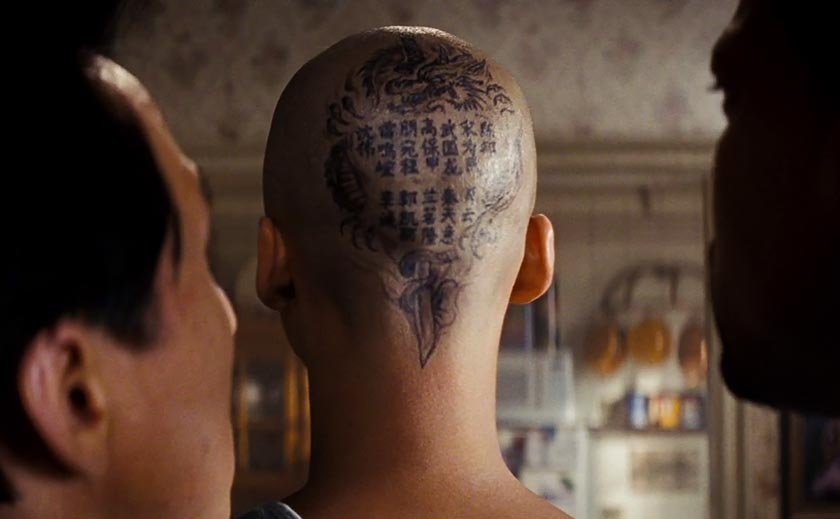
\includegraphics[width=6.5cm, height=4cm]{rushhour3nl11}\caption{scraping to the head}
        \onslide<2>\centering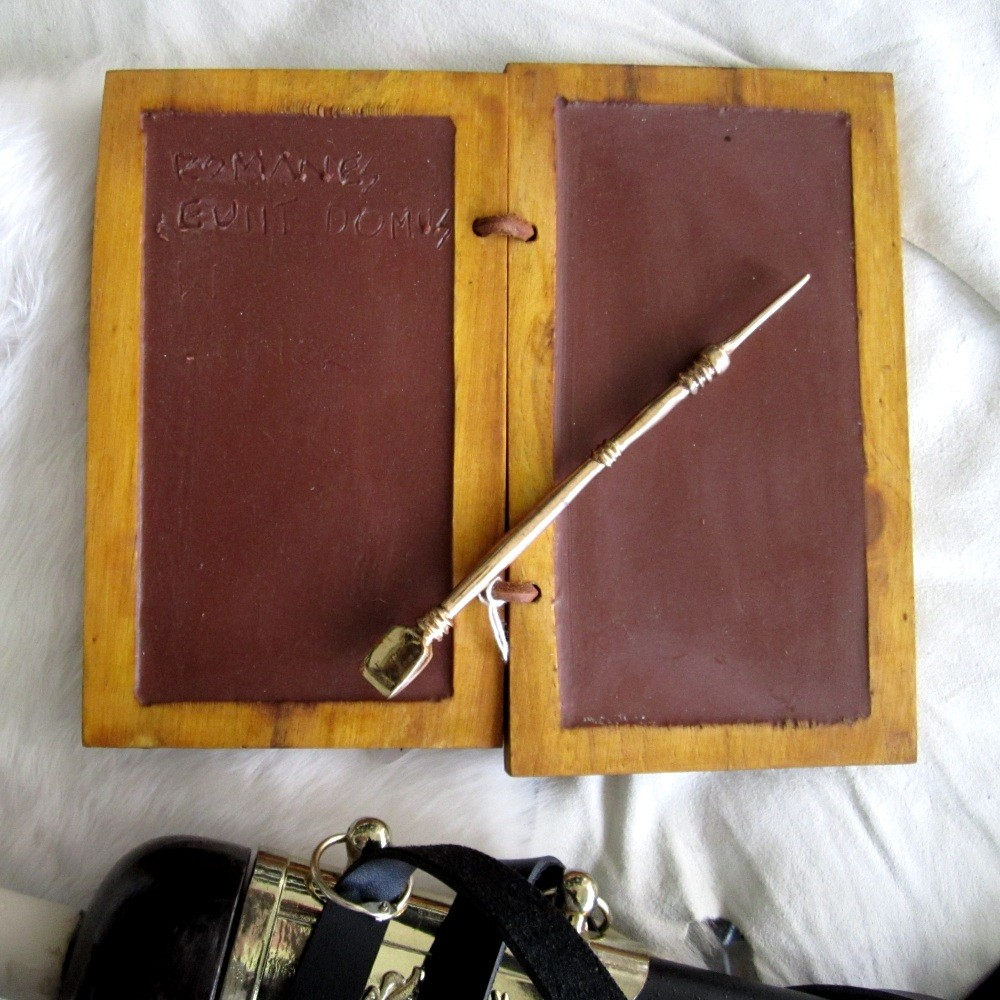
\includegraphics[width=6cm, height=4cm]{WaxTablet}\caption{wax tablets}
        \onslide<3>\centering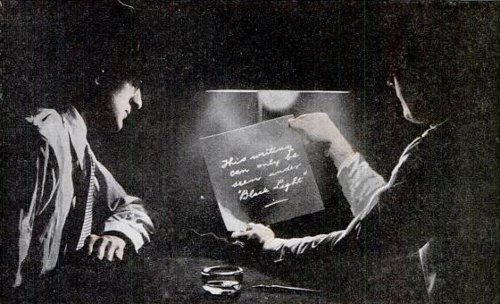
\includegraphics[width=6cm, height=4cm]{ink2.jpg}\caption{invisible ink}
        \onslide<4>\centering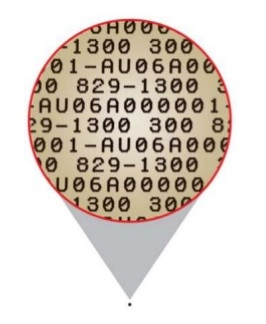
\includegraphics[width=4cm, height=5cm]{microdot.jpg}\caption{microdot technique}
        \onslide<5>\centering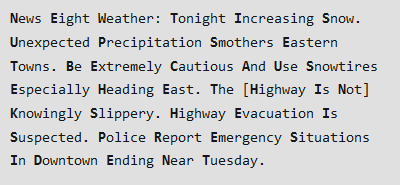
\includegraphics[width=6cm, height=4cm]{null}\caption{newtisupsetbecausehethinksheispresident}
        \onslide<6>\centering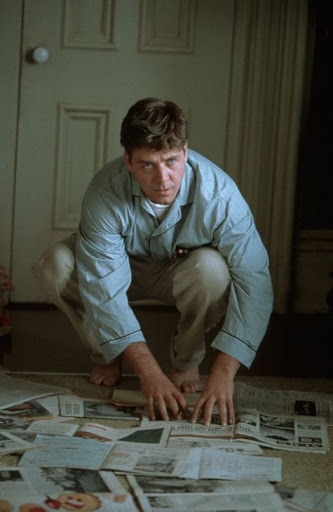
\includegraphics[width=3cm, height=5cm]{unnamed.jpg}\caption{In A Beautiful Mind, John Nash looks for hidden messages.}
    \end{overprint}
\end{figure}
\end{frame}

%-------------------------------
\subsection{Application Areas}
\begin{frame}
\frametitle{Application Areas}
Steganography is in the digital world. \\
\begin{figure}[h]
\centering

\includegraphics[width=8cm, height=5cm]{digital.png}
\end{figure}
%Over the World; texts, picture, sounds, video files are sent and received both compressed and uncompressed with the Internet.\\
%Today, there are multiple data hiding methods.\\
\end{frame}

%-------------------------------
\begin{frame}
\frametitle{Application Areas}
Steganography is done by deleting redundant and noisy data fields in file formats and replacing hidden messages.\\
\begin{figure}
    \centering
    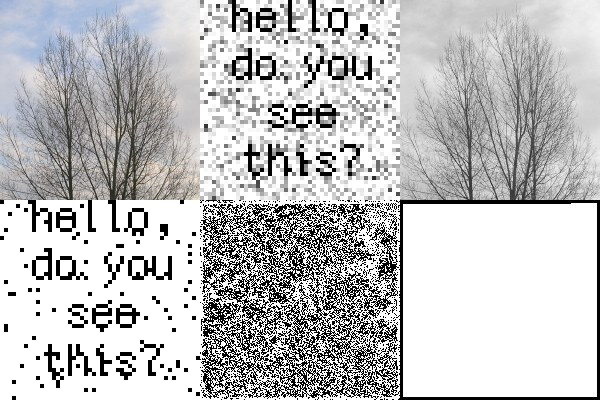
\includegraphics[width=8cm, height=5cm]{Embedding-Example.jpg}
   
    \label{}
\end{figure}
%The use of this method in the computer world is based on 2 main principles:
%\begin{itemize}
    %\item to embed data in the data
    %\item to hide the data in image or audio file
%\end{itemize}
\end{frame}

%-------------------------------
%\begin{frame}
%\frametitle{Application Areas}
%The content of the image or audio files can be changed to some degree without harming the image or %sound. \\
%The other principle is that the senses of a person cannot notice minor changes in image, sound or %color.
%\end{frame}

%-------------------------------
\begin{frame}
\frametitle{Application Areas}
When analyzing a steganographic algorithm, 3 main features should be considered:\\
\begin{itemize}
    \item Change should not be noticeable
    \item Amount of data that can be stored
    \item Durability
\end{itemize}

\end{frame}

%-------------------------------------
\subsection{Techniques}
\begin{frame}
\frametitle{Techniques}
The techniques used in steganography can be summarized as:\\
\begin{figure}[h]
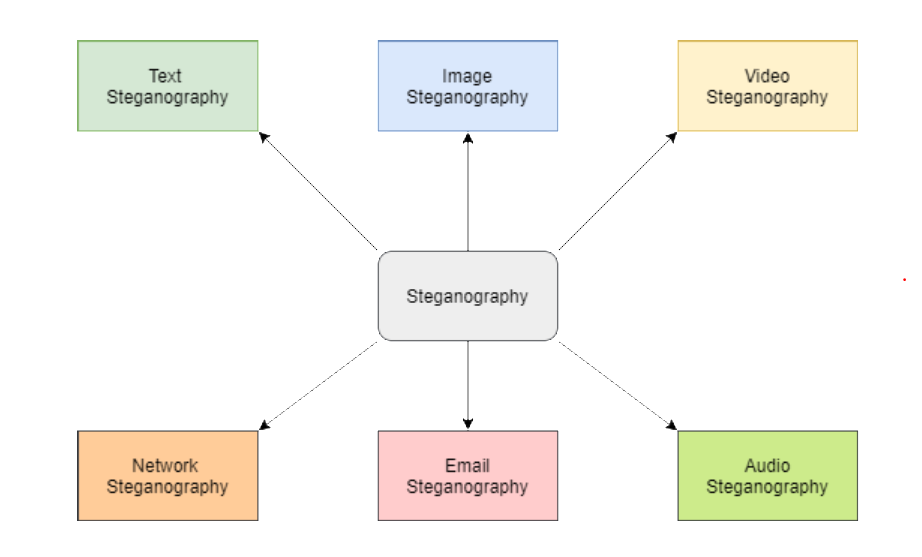
\includegraphics[width=10cm, height=6cm]{techniques.png}
\end{figure}
\end{frame}


%-------------------------------------
\subsection{Purpose, Significance \& Implications}
\begin{frame}
\frametitle{Purpose, Significance \& Implication}
\textbf{Purpose:} An environment using both cryptography and steganography.\\\pause
\textbf{Significance}: Steganography is not an alternative to encryption, but a complement to it.\\\pause
\textbf{Implications:} The development in steganography continues day by day, and its usage areas are open to expansion over time.
\end{frame}

%-------------------------------------
%\subsection{Significance}
%\begin{frame}
%\frametitle{Significance}
%Steganography is not an alternative to encryption, but a complement to it. \\
%This approach can be briefly described as hiding data inside an object.\\
%Audio, digital image or video files are used to hide encrypted data to further security.\\ 
%While encrypted data draw attention on their own, they will not be attempted to be broken because nobody will notice when they are hidden inside the image or audio files.
%\end{frame}

%-------------------------------------
%\subsection{Implications}
%\begin{frame}
%\frametitle{Implications}
%Steganography is a dynamic tool.\\
%Success in steganographic secrecy is achieved by choosing a suitable mechanism. 
%\\The development in steganography continues day by day, and its usage areas are open to %expansion over time. Its use will inspire many methods.

%\end{frame}
%%%%%%%%%%%%%%%%%%%%%%%%%%%%%%%%%%%%%%%
\section{Literature Review}
\begin{frame}
\frametitle{Literature Review}
Steganography and cryptography methods have been used  together. AES algorithm  have been used to encrypt the text to be sent, then embed this encrypted text in an image with the Least Significant Bit (LSB) method.\\\pause
RSA cryptosystem have also been used in another paper. \\\pause
In another paper, an architecture for information hiding in image steganography by using genetic algorithm and cryptography is proposed.\\\pause
Steganography based on complemented messages and inverted LSB substitution have been used.\\

\end{frame}
%-------------------------------------
%\begin{frame}
%\frametitle{Literature Review}
%M. Jain, S.K. Lenka and S.K. Vasistha have used RSA cryptosystem in adaptive circular queue image steganoraphy. The data structure queue is employed to resource distribution and RSA cryptosystem is used for secret information confidentiality and authentication. They get higher results as compared with several of existing algorithms of image steganography.\\

%\end{frame}

%-------------------------------------
%\begin{frame}
%\frametitle{Literature Review}
%In another paper, P.Sethi, V. Kapoor have proposed and architecture for information hiding in image steganography by using genetic algorithm and cryptography. \\
%R. Bhardwaj and V. Sharma have used steganography based on complemented messages and inverted LSB substitution where pixels are selected randomly when embedding the message.\\

%\end{frame}

%-------------------------------------
%\begin{frame}
%\frametitle{Literature Review}
%As it is seen in the literature, this study has a novel part. Finding a %way of combining different techniques from previous studies, is needed %to be done.
%
%\end{frame}

%%%%%%%%%%%%%%%%%%%%%%%%%%%%%%%%%%%%%%%
%\section{RSA \& AES}
%\subsection{RSA}
%\begin{frame}
%\frametitle{RSA}
%There are two types of encryption: symmetric and asymmetric encryption.\\
%Message between two people: Alice and Bob.\\
%Alice has a sensitive document that she wants to share with Bob. 
%\begin{figure}
%    \centering
%    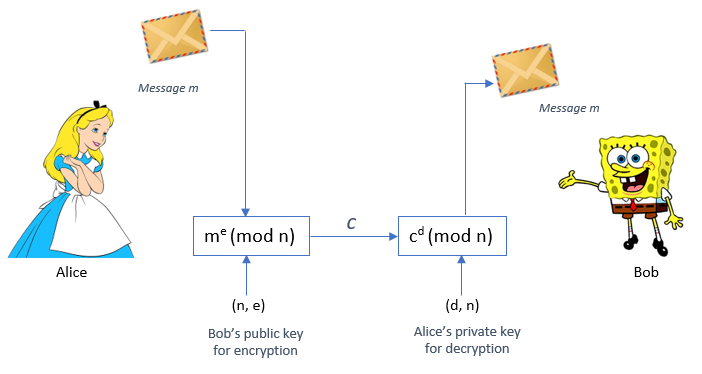
\includegraphics[width=9cm, height=4.5cm]{rsa.png}
%    \caption{}
%    \label{fig:my_label}
%\end{figure}
%\end{frame}

%-------------------------------------
%\begin{frame}
%\frametitle{RSA}
%RSA consists of three steps:\\
%\indent \textbf{1. Generating key}\\
%\indent \textbf{2. Message Encryption}\\
%\indent \textbf{3. Message Decryption}\\
%\end{frame}

%-------------------------------------
%\begin{frame}
%\frametitle{Generating key}
%\indent\indent • Two large enough prime numbers are selected, say %\textbf{p} and \textbf{q}.\\
%\indent\indent • \textbf{n} is computed as\textbf{ n=p.q}\\
%\indent\indent • Toitent function is computed as %\textbf{$\phi$(n)=(p-1).(q-1)}\\
%\indent\indent • A prime \textbf{e} number is selected such that %\textbf{gcd($\phi$, e)=1}
%and \textbf{1 $<$ e $<$ $\phi$}. \indent\indent   This \textbf{e} number is said to be the public key.\\
%\indent\indent • Then, a \textbf{d} number is computed as \textbf{d.e$\equiv$1 (mod $\phi$(n))}.  \\
%\indent\indent   Here the \textbf{d} number is said to be the private key.\\\\
%We have generated the keys. Now, we will encrypt the message.\\\\
%\end{frame}

%-------------------------------------
%\begin{frame}
%\frametitle{Message Encryption}
%\indent\indent • For encryption Bob sends his public key as %\textbf{(n,e)}.\\
%\indent\indent • Alice encrypts her message as %\textbf{c$\equiv$m$^{e}$(mod n)}\\\\
%\end{frame}

%-------------------------------------
%\begin{frame}
%\frametitle{Message Decryption}
%\indent\indent • For decrypt the message, Bob calculates %\textbf{m$\equiv$c$^{d}$(mod n)}, and gets message \textbf{m}. \\
%\end{frame}


%-------------------------------------
%\subsection{AES}
%\begin{frame}
%\frametitle{AES}
%AES is a “symmetric” encryption method, where the same secret (an encryption key) is used to encrypt the data, and also used to decrypt the data.\\
%\begin{center}
%\begin{figure}[!htbp]
%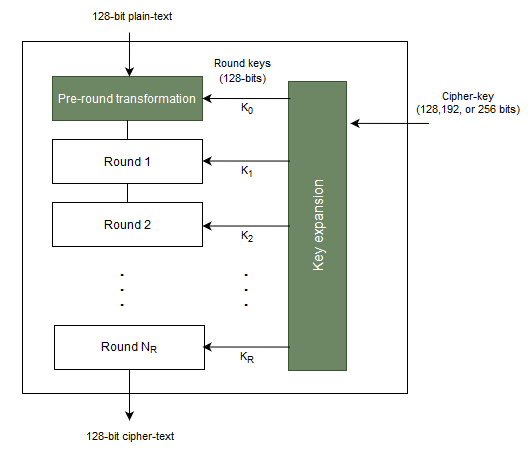
\includegraphics[width=7cm, height=5cm]{aes1.png}
%\centering
%\caption{AES Encryption Structure}
%\end{figure}
%\end{center}
%\end{frame}

%-------------------------------------
%\begin{frame}
%\frametitle{Encryption Process}
%Here is the typical description of round in AES encryption. Each round comprise of four sub-processes. The first round process is shown below:
%\begin{center}
%\begin{figure}[h]
%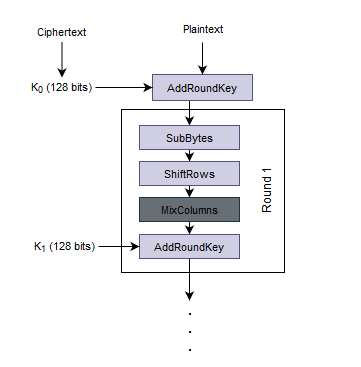
\includegraphics[width=6cm, height=5.5cm]{aes2}
%\centering
%\caption{AES Encryption Process of a Round}
%\end{figure}
%\end{center} 
%\end{frame}

%-------------------------------------
%\begin{frame}
%\frametitle{Byte Substitution (SubBytes)}
%The 16 input bytes are substituted by looking up a fixed table (S-box) %given in design. The result is a 4x4 matrix.\\
%\end{frame}


%-------------------------------------
%\begin{frame}
%\frametitle{Shiftrows}
%Each of the four rows of the matrix is shifted to the left. Any entries %that ‘fall off’ are re-inserted on the right side of row. Shift is carried out as follows:\\
%\begin{itemize}
    %\item First row is not shifted.
    %\item Second row is shifted one (byte) position to the left.
    %\item Third row is shifted two positions to the left.
    %\item Fourth row is shifted three positions to the left.
%\end{itemize}

   % The result is a new matrix consisting of the same 16 bytes but shifted with respect to each other.\\

%\end{frame}

%-------------------------------------
%\begin{frame}
%\frametitle{Mixcolumns}
%Each four-byte column is now converted using a special mathematical %function. This function takes four bytes of a column as input and %returns a completely new four byte that replaces the original column. %The result is another new matrix consisting of 16 new bytes. This step %was not carried out in the last round.\\
%\end{frame}

%-------------------------------------
%\begin{frame}
%\frametitle{AddRoundKey}
%The 16 bytes of the matrix are now considered as 128 bits and are converted to 128 bits of the round key with XOR. If this is the last round, the output is cipher text. Otherwise, the resulting 128 bits are interpreted as 16 bytes and we start another round.\\\\
%\end{frame}

%-------------------------------------
%\begin{frame}
%\frametitle{Decryption Process}
%\begin{center}
%\begin{figure}[h]
%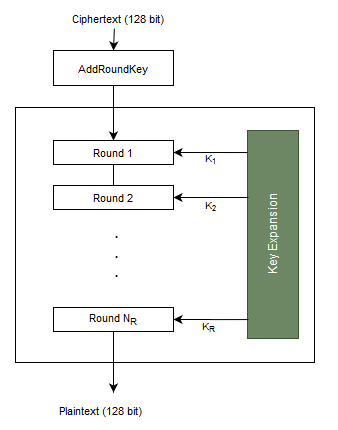
\includegraphics[width=7cm, height=7.5cm]{aes3}
%\centering
%\caption{AES Encryption Structure}
%\end{figure}
%\end{center}
%\end{frame}

%-------------------------------------
%\begin{frame}
%\frametitle{Decryption Process}
%The process of decryption of an AES is similar to the encryption process in the reverse order. Each round consists of the four processes in the reverse order:\\
%\begin{itemize}
 %   \item Add round key
 %   \item Mix columns
 %   \item Shift rows
 %   \item Byte substitution
%\end{itemize}
%\end{frame}

%-------------------------------------
%\begin{frame}
%\frametitle{Decryption Process}
%\begin{center}
%\begin{figure}[H]
%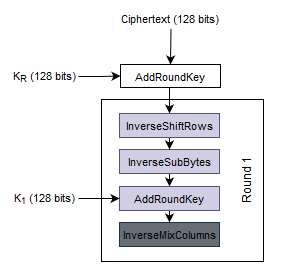
\includegraphics[width=4.5cm, height=4cm]{aes4}
%\centering
%\caption{AES Decryption Process of a Round}
%\end{figure}
%\end{center}
%\end{frame}

%%%%%%%%%%%%%%%%%%%%%%%%%%%%%%%%%%%%%%%
\section{Stegosystem \& Least Significant Bit (LSB)}
\begin{frame}
\frametitle{Stegosystem}
Formally a stegosystem consists of triplet that generates keys, encodes the message and decodes the message.\\
%\begin{itemize}
    %\item emb: message to be embedded
    %\item cover: file to embed the data
    %\item stego: modified version of the cover containing an embedded message
    %\item key: extra confidential data required for embedding and opening operations, which should also be known to the sender and receiver\\
%\end{itemize}
\begin{figure}[h]
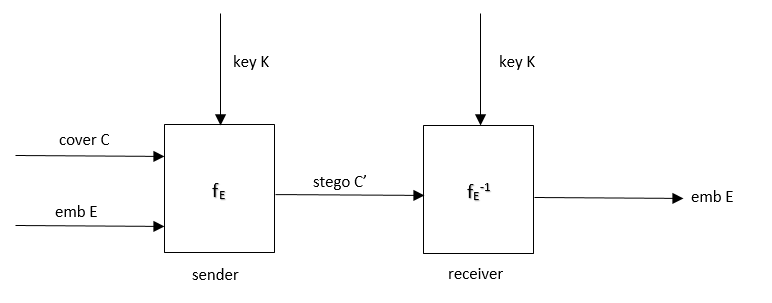
\includegraphics[width=12cm, height=4cm]{sego.png}
\centering
\caption{Formal Stegosystem}
\end{figure}
\end{frame}

%-------------------------------------
%\begin{frame}
%\frametitle{Least Significant Bit (LSB) Method}
%\begin{itemize}
    %\item f\textsubscript{E}: a steganographic function with key, emb and cover as parameter and generating stego as output
    %\item f\textsubscript{E}\textsuperscript{-1}: a steganographic function that has a stego with key as a parameter and generates emb as an output. f\textsubscript{E}\textsuperscript{-1} is the inverse function of f\textsubscript{E}.
%\end{itemize}
%\end{frame}

%-------------------------------------
%\begin{frame}
%\frametitle{Least Significant Bit (LSB) Method}
%\begin{figure}[h]
%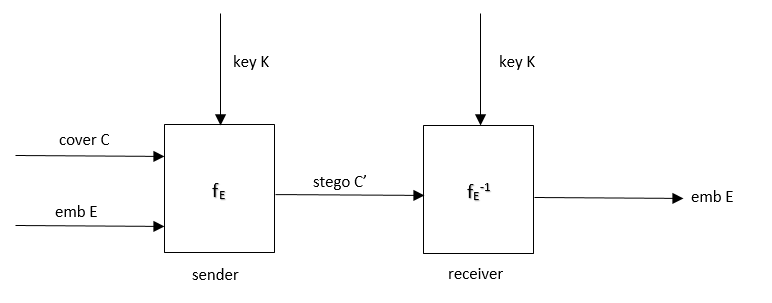
\includegraphics[width=12cm, height=4cm]{sego.png}
%\centering
%\caption{Formal Stegosystem}
%\end{figure}
%\end{frame}

%-------------------------------------
\begin{frame}
\frametitle{Stegosystem}
The sender creates a steganogram using a hiding function. The hiding function has two parameters, the carrier cover where the data will be stored and the data to be hidden.\pause
\begin{figure}[H]
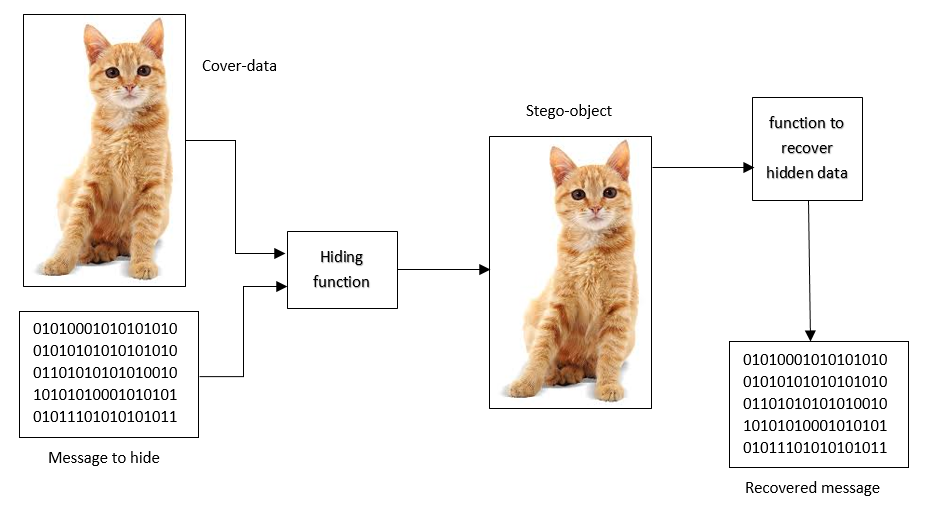
\includegraphics[width=11.5cm, height=5.5cm]{stego2.png}
\centering
\caption{Image Stegosystem}
\end{figure}
\end{frame}

%-------------------------------------
%\begin{frame}
%\frametitle{Stegosystem}
%\begin{figure}[H]
%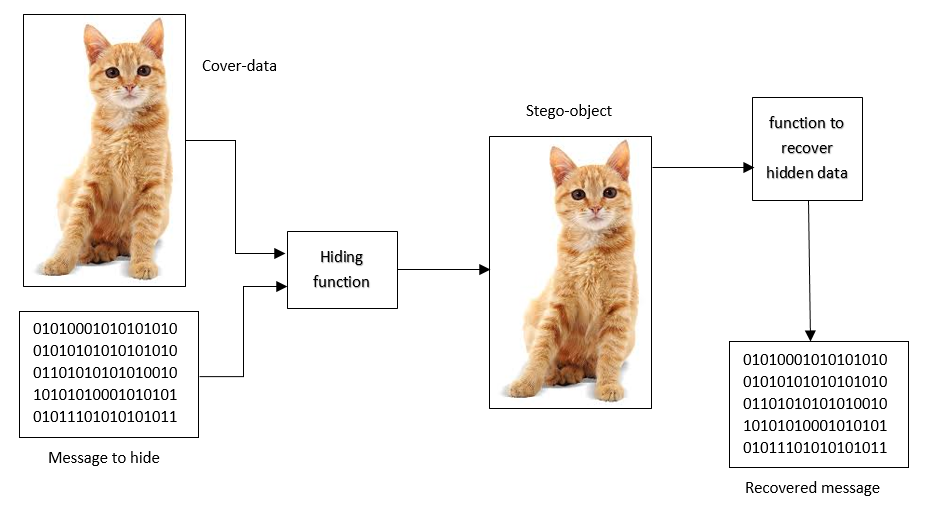
\includegraphics[width=11.5cm, height=5.5cm]{stego2.png}
%\centering
%\caption{Image Stegosystem}
%\end{figure}
%\end{frame}

%-------------------------------------
\begin{frame}
\frametitle{Hiding Functions}
In image steganography, there are various methods for hiding information in an image. These methods, called Hiding Function:\\
\begin{itemize}
    \item LSB
    \item Masking and Filtering
    \item Algorithms \& Transformations
\end{itemize} \\
\end{frame}

%-------------------------------------
\begin{frame}
\frametitle{RGB Channels}
\begin{figure}
    \begin{overprint}
        \onslide<1>\centering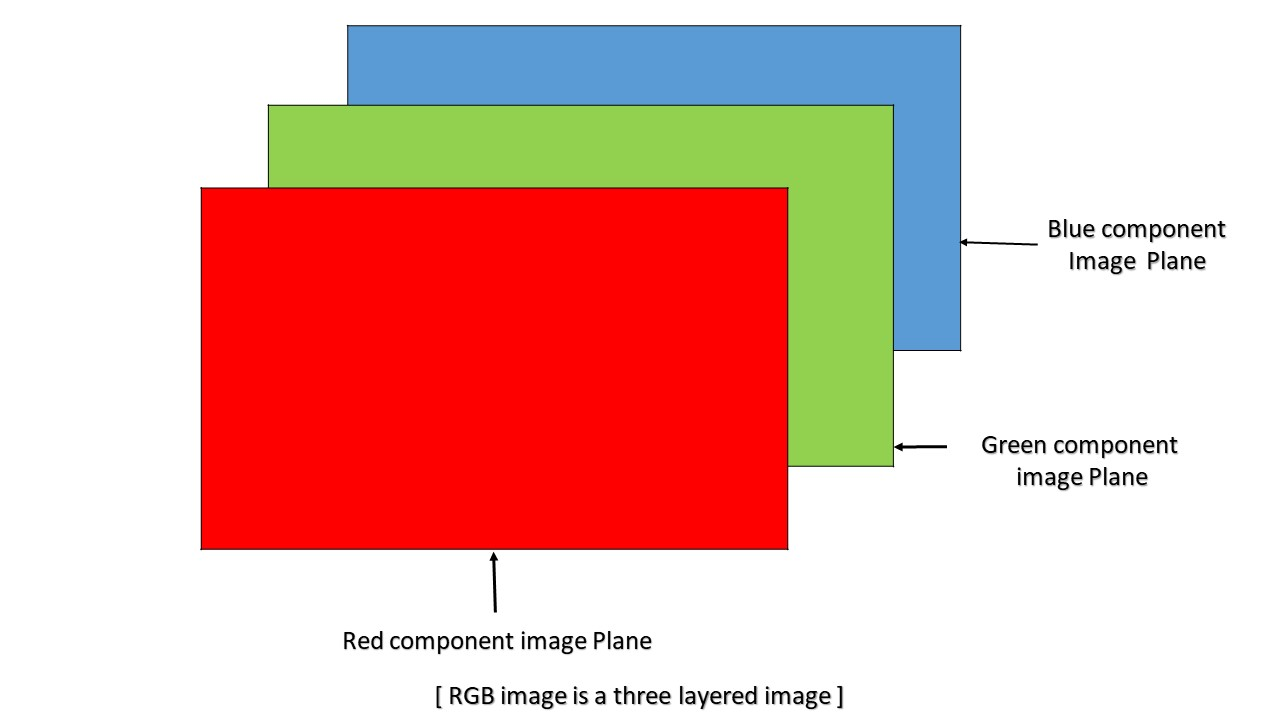
\includegraphics[width=9cm, height=5cm]{RGB-1.jpg}
        \onslide<2>\centering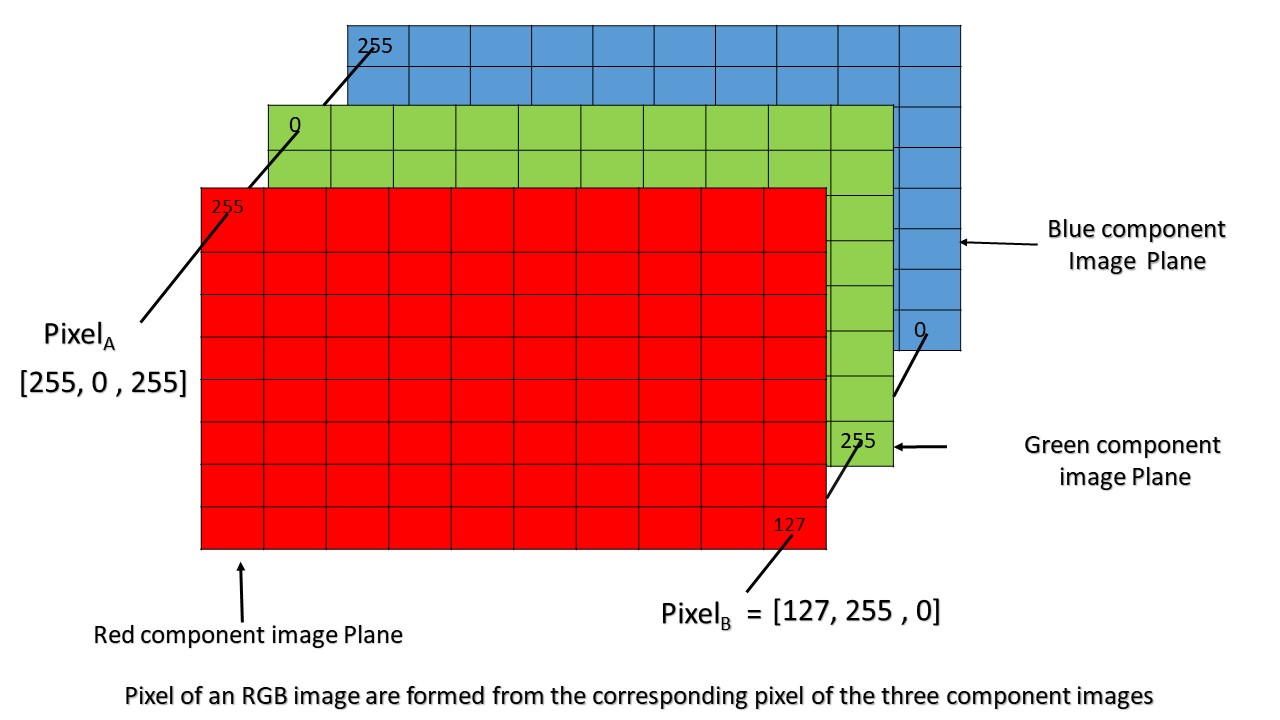
\includegraphics[width=9cm, height=5cm]{Pixel.jpg}
    \end{overprint}
\end{figure}
\end{frame}

%-------------------------------------
\begin{frame}
\frametitle{24-bit Image}
\begin{figure}[h]
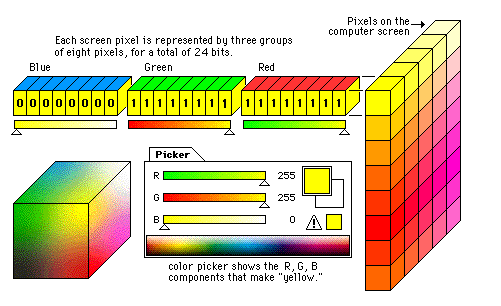
\includegraphics[width=10cm, height=5cm]{24bit.png}
\centering
\caption{Bitmap Colour Depth}
\end{figure}
\end{frame}

%-------------------------------------
\begin{frame}
\frametitle{Least Significant Bit (LSB) Method}
\begin{figure}
    \begin{overprint}
        \onslide<1>\centering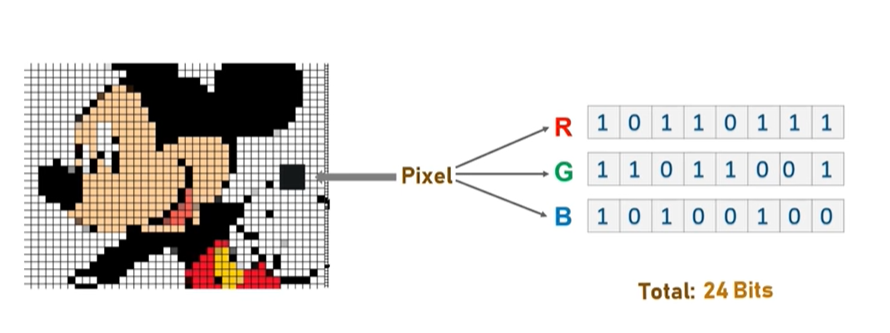
\includegraphics[width=11cm, height=5cm]{0 yARnljvGACzlItk-.png}
        \onslide<2>\centering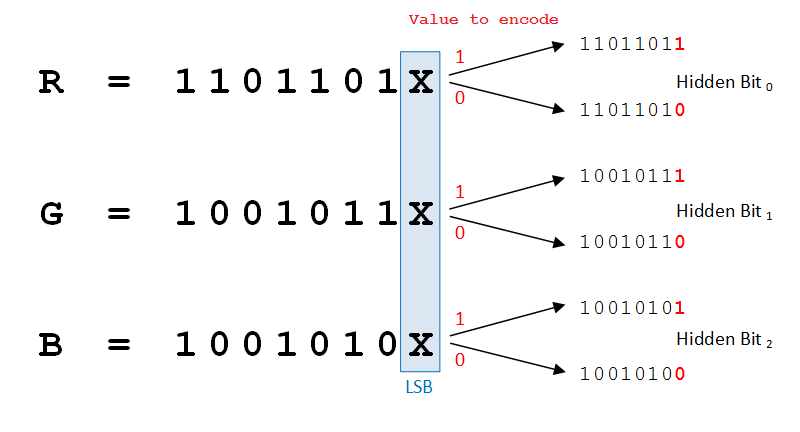
\includegraphics[width=10cm, height=5cm]{encode.png}
    \end{overprint}
\end{figure}
\end{frame}

%%%%%%%%%%%%%%%%%%%%%%%%%%%%%%%%%%%%%%%
\section{Methods Used In This Project}
\begin{frame}
\frametitle{Methods Used In This Project}

\begin{itemize}
    \item Least Significant Bit (LSB)
    \item Python programming language (back-end)
    \item OpenCV (Open Source Computer Vision Library)
    \item NumPy library
    \item docopt
    \item C\# (front-end)
\end{itemize}
\end{frame}
%-------------------------------------
\begin{frame}
\frametitle{Application}
\begin{figure}
    \centering
    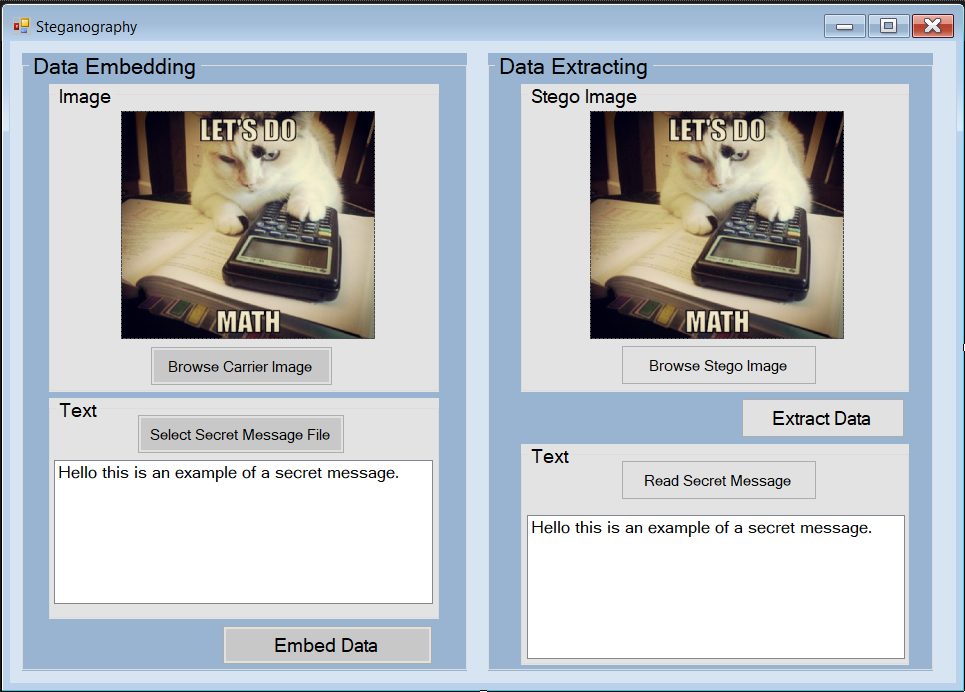
\includegraphics[width=10cm, height=7cm]{stego.png}
    \label{fig:my_label}
\end{figure}
\end{frame}

%-------------------------------------
%\begin{frame}
%\frametitle{Methods Used In This Project}
%As it is mentioned before, in this project LSB method has been used. This technique is using picture's pixel information.\\ This technique works best when the file is longer than the message file and if image is grayscale. When applying LSB techniques to each byte of a 24 bit image, three bits can be encoded into each pixel.\\
%\end{frame}


%-------------------------------------
\begin{frame}
\frametitle{Methods Used In This Project}
If the LSB of the pixel value of cover image C(i,j) is equal to the message bit SM of secret message to be embedded, C(i,j) remain unchanged; if not, set the LSB of C(i,j) to SM.\\
\end{frame}

%-------------------------------------
\begin{frame}
\frametitle{Message embedding procedure}
$$
S(i,j) = \left\{
        \begin{array}{ll}
            C(i,j)-1 & \quad $LSB(C(i,j))=1$ $ and$ $ SM=0$ \\
             C(i,j)+1 & \quad $LSB(C(i,j))=0$ $ and$ $ SM=1$ \\
              C(i,j) & \quad $LSB(C(i,j))=SM$
        \end{array}
    \right.
$$
where LSB(C(i,j)) stands for the LSB of the cover image C(i,j) and "SM" is the next message bit to be embedded. S(i,j) is the stego image.\\
\end{frame}

%-------------------------------------
%\begin{frame}
%\frametitle{Algorithm Used in the Code for Embedding}
%\begin{itemize}
%\item Step 1: Extract the pixels of the cover image.
%\item Step 2: Extract the character of the text or the pixels of the image.
%\item Step 3: Extract the length of the secret message. (Length coded on 2 bytes so the text size can be up to 65536 bytes long)
%\item Step 4: Choose first pixel and embed length of the secret message in the first 2 bytes pixels.
%\item Step 5: Skip to the pixels after the length bytes.
%\item Step 6: Insert characters of the message text in each component of next pixels by replacing it.
%\item Step 7: Repeat step 6 till all the characters has been embedded.\\\\
%\end{itemize}
%\end{frame}

%-------------------------------------
\begin{frame}
\frametitle{Message extracting procedure}
$$
SM = \left\{
        \begin{array}{ll}
            0  & \quad $S(i,j)=0$\\
            1  & \quad $S(i,j)=1$ 
        \end{array}
    \right.
$$
where "SM" is the message bit has been embedded. S(i,j) is the stego image.\\
\end{frame}

%-------------------------------------
%\begin{frame}
%\frametitle{Data Extracting Procedure}
%\begin{itemize}
%\item Step 1: Extract the pixels of the stego image.
%\item Step 2: Start from first pixel and extract length of the message from first 2 bytes components of the pixels. 
%\item Step 3: Skip to the pixels after the length bytes.
%\item Step 4: Extract secret message bits from the pixels.
%\item Step 5: Repeat step 4 till reach the pixels of length of the message.
%\item Step 6: Decode message.
%\end{itemize}
%Here, every 4 bit-block represents an ASCII character, so it is easy to decode from ASCII to message character.
%\end{frame}




%%%%%%%%%%%%%%%%%%%%%%%%%%%%%%%%%%%%%%%
\section{Conclusion \& Discussion}
\begin{frame}
\frametitle{Conclusion \& Discussion}


The work proposed in this presentation can be summarized with the following points:\\
\begin{itemize}
\pause
\item Steganography and its history with old methods have been presented. 
\item The application areas for steganography has been mentioned.
%\item Some techniques used for steganography have been listed.
\item Purpose, significance and implications of this project have been discussed.

\end{itemize}
\end{frame}
%----------------------------------------------------------

\begin{frame}
\frametitle{Conclusion \& Discussion}

\begin{itemize}
\item Some literature review has done. %4 papers have been mentioned and these papers are about using steganography with cryptography.
%\item RSA and AES have been explained with their basic principles.
\item Least Significant Bit (LSB) method explained basically.
\item Methods used in this project have been summarized. %and finally a conclusion and discussion part have been placed in this report.
\end{itemize}
\end{frame}
%----------------------------------------------------------
\begin{frame}
\frametitle{Conclusion \& Discussion}
\begin{centering}
In this project, I wanted to use steganography with cryptography methods, but up to this time I have not been able to combine these two methods. So, this is left as a future work from now on. But LSB method for secret text/image embedding into an image worked properly.
\end{centering}
\end{frame}
%----------------------------------------------------------
\begin{frame}
\begin{centering}THANK YOU FOR LISTENING!\\\end{centering}
\begin{centering}Any questions?\\\end{centering}

\end{frame}
\end{document}
